% This must be in the first 5 lines to tell arXiv to use pdfLaTeX, which is strongly recommended.
\pdfoutput=1
% In particular, the hyperref package requires pdfLaTeX in order to break URLs across lines.

\documentclass[11pt]{article}

% Remove the "review" option to generate the final version.
\usepackage[review]{EMNLP2023}

% Standard package includes
\usepackage{times}
\usepackage{latexsym}
\usepackage{float}

% For proper rendering and hyphenation of words containing Latin characters (including in bib files)
\usepackage[T1]{fontenc}
% For Vietnamese characters
% \usepackage[T5]{fontenc}
% See https://www.latex-project.org/help/documentation/encguide.pdf for other character sets

% This assumes your files are encoded as UTF8
\usepackage[utf8]{inputenc}

% This is not strictly necessary, and may be commented out.
% However, it will improve the layout of the manuscript,
% and will typically save some space.
\usepackage{microtype}

% This is also not strictly necessary, and may be commented out.
% However, it will improve the aesthetics of text in
% the typewriter font.
\usepackage{inconsolata}
% includegraphics
\usepackage{graphicx}
%listings
\usepackage{listings}
\usepackage{dirtytalk}
\usepackage{enumitem}
\usepackage{graphicx}
\usepackage{array}
\usepackage{booktabs}
%review macros
\usepackage{xcolor}
\newcommand{\review}[1]{{\color{black}#1}}

%pandas tables
\usepackage{{booktabs}}
% Commands
\newcommand{\todo}[1]{{\color{red}\colorbox{yellow}{\textbf{TODO: }}#1}}
\newcommand{\averitec}{FEVER~8}
\newcommand{\evr}{Ev\textsuperscript{2}R}
\newcommand{\supp}{Supported}
\newcommand{\reff}{Refuted}
\newcommand{\nei}{Not enough evidence}
\newcommand{\conf}{Conflicting evidence/Cherrypicking}
\makeatletter
\newcommand\footnoteref[1]{\protected@xdef\@thefnmark{\ref{#1}}\@footnotemark}
\makeatother

% If the title and author information does not fit in the area allocated, uncomment the following
%
%\setlength\titlebox{<dim>}
%
% and set <dim> to something 5cm or larger.

\title{AIC CTU@FEVER 8: On-premise fact checking through long context RAG}

% Author information can be set in various styles:
% For several authors from the same institution:
% \author{Author 1 \and ... \and Author n \\
%         Address line \\ ... \\ Address line}
% if the names do not fit well on one line use
%         Author 1 \\ {\bf Author 2} \\ ... \\ {\bf Author n} \\
% For authors from different institutions:
% \author{Author 1 \\ Address line \\  ... \\ Address line
%         \And  ... \And
%         Author n \\ Address line \\ ... \\ Address line}
% To start a seperate ``row'' of authors use \AND, as in
% \author{Author 1 \\ Address line \\  ... \\ Address line
%         \AND
%         Author 2 \\ Address line \\ ... \\ Address line \And
%         Author 3 \\ Address line \\ ... \\ Address line}

\author{Herbert Ullrich \\
AI Center @ CTU FEE\\
Charles Square 13\\
Prague, Czech Republic\\
\texttt{ullriher@fel.cvut.cz} \\\And
Jan Drchal \\
AI Center @ CTU FEE\\
Charles Square 13\\
Prague, Czech Republic\\
\texttt{drchajan@fel.cvut.cz} \\}

\begin{document}
{\makeatletter\acl@finalcopytrue
  \maketitle
}
\begin{abstract}
In this paper, we present our fact-checking pipeline which has scored first in \averitec{} shared task. Our fact-checking system is a simple two-step RAG pipeline based on our last year's submission. We show how the pipeline can be redeployed on-premise, achieving state-of-the-art fact-checking performance (in sense of \evr{} test-score), even under the constraint of a single Nvidia A10 GPU, 23GB of graphical memory and 60s running time per claim.

\end{abstract}

%%%%%%%%%%%%%%%%%%%%%%%%%%%%%%%%%%%%
% inputs
%!TEX ROOT=../emnlp2023.tex

% show figures/pipeline.png
\begin{figure}[h]
    \centering
    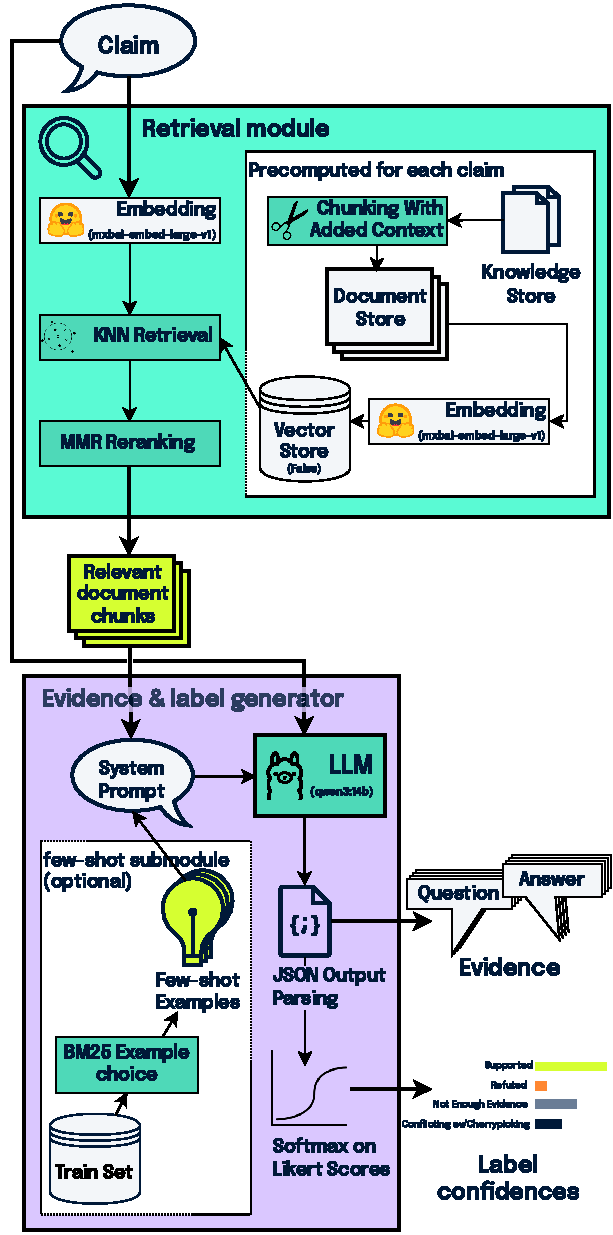
\includegraphics[width=0.45\textwidth]{figures/pipeline.pdf}
    \caption{Our refreshed pipeline, adapted from TODO}
    \label{fig:pipeline}
\end{figure}

\section{Introduction}
\label{sec:introduction}


\section{Related work}
\label{sec:relwork}
\label{avscore}
\begin{enumerate}
    \item \textbf{\averitec{} shared task}~\cite{averitec2024} releases the datase of real-world fact-checked claims, annotated with evidence available at the date the claim was made.
\end{enumerate}


%!TEX ROOT=../emnlp2023.tex

\section{System description}
\label{sec:system}

Our system is a straightforward adaptation of the AIC CTU Averitec system designed one year prior, published in~\citealt{ullrich-etal-2024-aic}.
The cited paper describes the system in detail, with ablation studies and justifications of each step.
Our pipeline, depicted in Figure~\ref{fig:pipeline}, consists of precomputation, retrieval, and generation modules:

\begin{enumerate}[label=\roman*.]  % First-level: i., ii., iii.
\item Precomputation module
\begin{enumerate}[label=\arabic*.]  % Second-level: 1., 2., 3.
    \item The provided AVeriTeC \textbf{knowledge store} \cite{averitec2024} is split into chunks of specified maximum length, each marked with metadata of its URL and the full texts of the chunk before and after.
    \item The chunks are then embedded into their vector representations, using only the chunk texts and no metadata.
    \item Out of all chunk embeddings, a \textbf{vector store} is produced for each claim to be stored as a vector database.
\end{enumerate}
\item Retrieval module
\begin{enumerate}[label=\arabic*.]  % Second-level: 1., 2., 3.
    \item The \textbf{Claim} is embedded into its vector representation using the same model used in i.2.
    \item $k$ nearest neighbours are then retrieved from the vector store, along with their \textbf{chunk embeddings}
    \item The chunk embeddings are then re-ranked using the Maximal Marginal Relevance (MMR) method~\cite{carbonell-mmr}, maximizing the embedding distances between retrieval results while minimizing their distance to the claim.
    Ultimately, we output a subset of $l$~diverse \textbf{sources} for the claim ($l<k$), augmenting each with its context before, after, and the text of its URL.
\end{enumerate}
\item Evidence \& label generation module
\begin{enumerate}[label=\arabic*.]  % Second-level: 1., 2., 3.
    \item We instruct a Large Language Model (LLM) to produce Question-Answer pairs required to fact-check given claim based on the provided sources, and predict its veracity verdict in a single output. We pass it the texts of all $l$ sources, and several few-shot QA-pair generation examples picked from Averitec train set using BM25. The whole instruction is serialized into a system prompt and the format we used can be seen in Appendix~\ref{appendix_sec:system_prompt}.
    \item \textbf{Claim} is then passed to the LLM as a user message.
    \item LLM is called to \textbf{generate the evidence} as a Question-Answer-Source triples and the Likert-scale scores for each possible \textbf{veracity verdict} in a single prediction, performing a chain of thought. 
    \item The LLM output is parsed, and the verdict with the highest score is chosen for the claim.
\end{enumerate}
\end{enumerate}

The main differences between this year's AIC \averitec{} system, opposed to last year's AIC AVeriTeC system, are the omission of knowledge store pruning in the precomputation step\footnote{The precomputed vector stores were required to be independent on claim text in \averitec{}.}, and, importantly, the choice of LLM.
\subsection{Model and parameter choices}
\label{sec:choices}
To produce our submission in the \averitec{} shared task, the following choices were made to deploy the pipeline from section~\ref{sec:system}:

\texttt{mxbai-embed-large-v1}~\cite{li-li-2024-aoe,emb2024mxbai} is used for the vector embeddings, and the maximum chunk size is set to 2048 characters, considering its input size of 512 tokens and a rule-of-thumb coeffitient of 4 characters per token to exploit the full embedding input size and produce the smallest possible vector store size without neglecting a significant proportion of knowledge store text.

\texttt{FAISS}~\cite{douze2024faiss,johnson2019billion} index is used as the vector database engine, due to its simplicity of usage, exact search feature and quick retrieval times (sub-second for a single \averitec{} test claim).

$l=10, k=40, \lambda=0.75$ are the parameters we use for the MMR reranking, meaning that 40 chunks are retrieved, 10 sources are to yielded, and the tradeoff between their similarity to the claim and their diversity is 3:1 in favour of the source similarity to the claim (explained in more detail in~\citealt{ullrich-etal-2024-aic}). 

\texttt{Ollama} wrapper around \texttt{llama.cpp} is the LLM engine we use to deploy LLMs within the \averitec~test environment due to its robustness and ease of deployment.

\texttt{Qwen3-14b}~\cite{yang2025qwen3technicalreport} is the LLM we use to produce the evidence and labels, we also let it generate its own \texttt{<think>} sequences, although further experimentation (Table~\ref{tab:ablation}) suggests that the thinking tokens may not justify the costs of their prediction, as they seem to perform on par with using only the evidence \& label LLM outputs for a chain of thought.
%\input{src/classification}
%!TEX ROOT=../emnlp2023.tex

\section{Results and analysis}
\label{sec:results}
\label{nothink}

\subsection{Why does the system perform well?}
\label{sec:why}
One thing we would like to address with this paper is why does our system outperform the \averitec{} baseline and even the other systems submitted to \averitec{} shared task despite the simplicity of its design (Figure~\ref{fig:pipeline}) which boils down to a straightforward case of retrieval-augmented generation (RAG).

The main reason, in our experience, is the large \textbf{context size} we opt for -- while even the \averitec{} baseline processes the claims and sources in a manner more sophisticated than we do, it processes the knowledge store on a \textit{sentence} level, reducing the amount of information passed to the LLM as opposed to working with \textit{documents} as a whole, which is the strategy our system approximates.

Put simply, despite our integration of LLM into the pipeline being rather vanilla, providing the model with retrieved sources of combined length of around 60K characters\footnote{In other words, around 33 standard pages. This number follows from our parameter choices in Section~\ref{sec:choices}: 10 chunks of $\sim2048$ characters and additional $\sim4096$ characters of context each.} yields highly competitive results, leveraging its own trained mechanisms of context processing.

Our other advantages may have been using a very recent model, Qwen3~\cite{yang2025qwen3technicalreport}, which naturally has a slightly higher leakage of 2025 claims into its train set than older models, and outperforms the previous LLM generations at long sequence processing. Furthermore, our pipeline design only uses a single LLM call per claim, meaning we could use the generously-sized 14B variant of Qwen3 and still match the time limit with Nvidia A10 and 20GB GRAM.
%\input{src/software.tex}
%!TEX ROOT=../emnlp2023.tex

\section{Conclusion}
\label{sec:conclusion}


\subsection{Future works}
\begin{enumerate}
    \item Integrating a search API for use in \review{real-world applications} 
    
\end{enumerate}

%%%%%%%%%%%%%%%%%%%%%%%%%%%%%%%%%%%%

\section*{Limitations}
Our pipeline is not meant to be relied upon nor to replace a human fact-checker, but rather to assist an informed user. It gives sources and proposed labels for further questioning. It is optimized only for English, the carbon costs of the used models are considerable, despite the system trying to cut down the environmental cost of the prediction step.

\section*{Ethics statement}
Our pipeline is an extension of our already existing last year submission all original authors agreed with, including the reusal of the necessary listing in Appendix~\ref{appendix_sec:system_prompt}.
The system was build specifically for the~\averitec~shared task and reflects the biases of its annotators, for more information on this, we suggest the original AVeriTeC paper~\cite{averitec2024}.
\section*{Acknowledgements}
This article was created with the state support of the Ministry of Industry and Trade of the Czech Republic, project no. Z220312000000, within the National Recovery Plan Programme.
The access to the computational infrastructure of the OP VVV funded project CZ.02.1.01/0.0/0.0/16\_019/0000765 ``Research Center for Informatics'' is also gratefully acknowledged.



% Entries for the entire Anthology, followed by custom entries
\bibliography{anthology,custom}
\bibliographystyle{acl_natbib}

\appendix

%!TEX ROOT=../emnlp2023.tex


\lstset{
    language={},
    basicstyle=\ttfamily\footnotesize\linespread{0.9}, % Smaller font with less spacing
    keywordstyle=\color{blue}\bfseries,
    commentstyle=\color{green!50!black}\itshape,
    stringstyle=\color{orange},
    numberstyle=\tiny\color{gray},
    numbers=none, % Line numbers on the left
    stepnumber=1, % Line numbers for every line
    numbersep=5pt, % Space between line numbers and code
    tabsize=4, % Size of tabs
    showstringspaces=false, % Don't show spaces in strings
    breaklines=true, % Line wrapping
    breakatwhitespace=true,
    frame=lines, % Add a frame around the code
    captionpos=b, % Caption at the 
    breakindent=1em,
}
\begin{figure*}
    \section{System prompt}
    \label{appendix_sec:system_prompt}
    \begin{lstlisting}[breaklines=true, language={}, frame=single, caption={System prompt for the LLMs, \averitec{} claim is to be entered into the user prompt. Three dots represent omitted repeating parts of the prompt. Reused from~\citealt{ullrich-etal-2024-aic}.}, label={lst:llm_system_prompt}]
You are a professional fact checker, formulate up to 10 questions that cover all the facts needed to validate whether the factual statement (in User message) is true, false, uncertain or a matter of opinion. Each question has one of four answer types: Boolean, Extractive, Abstractive and Unanswerable using the provided sources.
After formulating Your questions and their answers using the provided sources, You evaluate the possible veracity verdicts (Supported claim, Refuted claim, Not enough evidence, or Conflicting evidence/Cherrypicking) given your claim and evidence on a Likert scale (1 - Strongly disagree, 2 - Disagree, 3 - Neutral, 4 - Agree, 5 - Strongly agree). Ultimately, you note the single likeliest veracity verdict according to your best knowledge.
The facts must be coming from these sources, please refer them using assigned IDs:
---
## Source ID: 1 [url]
[context before]
[page content]
[context after]
...

---
## Output formatting
Please, you MUST only print the output in the following output format:
```json
{
 "questions":
     [
         {"question": "<Your first question>", "answer": "<The answer to the Your first question>", "source": "<Single numeric source ID backing the answer for Your first question>", "answer_type":"<The type of first answer>"},
         {"question": "<Your second question>", "answer": "<The answer to the Your second question>", "source": "<Single numeric Source ID backing the answer for Your second question>", "answer_type":"<The type of second answer>"}
     ],
 "claim_veracity": {
     "Supported": "<Likert-scale rating of how much You agree with the 'Supported' veracity classification>",
     "Refuted": "<Likert-scale rating of how much You agree with the 'Refuted' veracity classification>",
     "Not Enough Evidence": "<Likert-scale rating of how much You agree with the 'Not Enough Evidence' veracity classification>",
     "Conflicting Evidence/Cherrypicking": "<Likert-scale rating of how much You agree with the 'Conflicting Evidence/Cherrypicking' veracity classification>"
 },
 "veracity_verdict": "<The suggested veracity classification for the claim>"
}
```
---
## Few-shot learning
You have access to the following few-shot learning examples for questions and answers.:

### Question examples for claim "{example["claim"]}" (verdict {example["gold_label"]})
"question": "{question}", "answer": "{answer}", "answer_type": "{answer_type}"
...
    \end{lstlisting}
\end{figure*}
%!TEX ROOT=../emnlp2023.tex

\label{appendix_sec:think}


\lstset{
    language={},
    basicstyle=\ttfamily\footnotesize\linespread{0.9}, % Smaller font with less spacing
    keywordstyle=\color{blue}\bfseries,
    commentstyle=\color{green!50!black}\itshape,
    stringstyle=\color{orange},
    numberstyle=\tiny\color{gray},
    numbers=none, % Line numbers on the left
    stepnumber=1, % Line numbers for every line
    numbersep=5pt, % Space between line numbers and code
    tabsize=4, % Size of tabs
    showstringspaces=false, % Don't show spaces in strings
    breaklines=true, % Line wrapping
    breakatwhitespace=true,
    frame=lines, % Add a frame around the code
    captionpos=b, % Caption at the 
    breakindent=1em,
}
\begin{figure*}
    \section{Qwen3 thinking example}
    \label{appendix_sec:think}
    \begin{lstlisting}[breaklines=true, language={}, frame=single, caption={Qwen3 thinking tokens example.}, label={lst:think}]
<think>
Okay, let's tackle this query. The user is claiming that due to Imran Khan's criticism of Macron's comments on Islam, French authorities cancelled the visas of 183 Pakistani citizens and deported 118 from the country. I need to verify this using the provided sources.

First, I'll look through the sources to see if there's any mention of visa cancellations or deportations related to Imran Khan's criticism. 

Looking at Source ID 1, it talks about Imran Khan responding to Macron's remarks and the condemnation of Islamophobic policies, but there's no mention of visa cancellations or deportations. 

Source ID 2 discusses a diplomatic row where Pakistan refused to accept a deportee, Muhammad Mansha, until his credentials were verified. This seems related to a specific case but not the large numbers mentioned in the claim.

Source ID 3 mentions protests in Pakistan against France's republishing of cartoons, but again, no visa or deportation numbers here.

Source ID 4 and 5 discuss diplomatic tensions, but not specific numbers of deportations. Source 5 and 6 from Newscomworld.com talk about fears of deportations of Pakistanis in France but don't mention specific numbers like 183 or 118.

Source ID 7 is about Pakistan deporting French nationals, which is the reverse of the claim. 

Source ID 10 mentions Pakistan summoning the French envoy but again, no numbers on deportations.

None of the sources mention 183 visas cancelled or 118 deported. The closest is Source 2, which mentions one individual, Muhammad Mansha, but that's a single case. The other sources discuss diplomatic tensions, protests, and possible fears of deportations but no actual numbers provided. 

Therefore, the claim about 183 and 118 seems to be unsupported. The answer would be that there's no evidence of such numbers in the sources provided. The veracity verdict would be Refuted, as the sources don't support the specific numbers given.
</think>

```json
{
    "questions": [
        {"question": "Did French authorities cancel visas or deport Pakistani citizens in response to Imran Khan's criticism of Macron's comments on Islam?", "answer": "No specific information about visa cancellations or deportations of 183 Pakistani citizens or 118 deportees is mentioned in the provided sources.", "source": "10", "answer_type": "Boolean"},
        ...
        {"question": "What was the role of social media in the diplomatic dispute between Pakistan and France?", "answer": "Social media was used to spread calls for boycotts of French products and even nuclear attacks on France, but these were not confirmed by official sources.", "source": "5", "answer_type": "Extractive"}
    ],
    "claim_veracity": {
        "Supported": "1",
        "Refuted": "5",
        "Not Enough Evidence": "1",
        "Conflicting Evidence/Cherrypicking": "1"
    },
    "veracity_verdict": "Refuted"
}
```
    \end{lstlisting}
\end{figure*}
%\include{src/appendix_b_opensource}
%\include{src/appendix_c_errors}

\end{document}
